\section{Equilibrium characterization}
\label{sec:rewrite-regimes}

In this section, I give sufficient conditions for the existence of an equilibrium and characterize the long-run behavior of these equilibria for various parameter configurations. The key finding is that long-run output-per-worker growth can exceed the rate of labor-augmenting technological change when the elasticity of substitution between AI production services and labor exceeds one and the upper bound on AI efficiency is sufficiently high.

To identify this threshold, I calculate the net return on capital implied by the production and pricing conditions as AI efficiency approaches its upper bound and labor's income share tends to zero. I compare this return with $\rho+\gamma$, the interest rate that sustains consumption-per-person growth at the exogenous rate $\gamma$. When AI and labor are substitutes and the former return exceeds the latter, the model supports equilibrium paths along which capital and AI production services grow faster than effective labor, even though AI efficiency converges to a finite limit.
%The parameter restrictions used in all three propositions are
%\begin{equation}
% \begin{gathered}
% 0<\alpha<1,\quad 0<\eta<1,\quad \delta\geq0,\quad \chi>0,\\
% \omega_L,\omega_X>0,\quad \omega_L+\omega_X=1,\quad
% n\geq0,\quad \gamma>0,\quad \rho>n.
% \end{gathered}
% \label{eq:rewrite-finite-existence-parameters}
%\end{equation}
%These are the primitive restrictions in Section~\ref{sec:rewrite-model}.
%In particular, the local finite-frontier results do not require Assumptions~\ref{ass:rewrite-research-curvature} or \ref{ass:rewrite-research-concavity}. Sufficiently near the frontier, its diminishing scope for improvement permits global verification of the developer's policy even when $\eta>1/2$.

%The inequality $n+\gamma>0$ already follows from \eqref{eq:rewrite-population} and \eqref{eq:rewrite-labor-productivity}, so it is not a separate assumption. It makes effective labor grow and gives the remaining AI-efficiency gap a positive asymptotic rate of closure in the constructions below. The case $n+\gamma=0$ is not covered by these proofs.

%Each proposition below states the restrictions on $\sigma$, the frontier, and the initial stocks that are specific to its construction. The results do not concern the uncapped economy. They are local in initial stocks, not in time: each constructs a trajectory defined for every $t\geq0$, including both transversality conditions and agent optimality. The initial stocks need not lie on a balanced-growth path. The neighborhoods are in normalized coordinates and require initial AI efficiency sufficiently close to its frontier. Local uniqueness below means uniqueness among solutions that remain near the indicated normalized long-run limit and converge to it; it does not exclude other equilibria outside that neighborhood.

\subsection{The return to capital and the efficiency threshold}
\label{subsec:rewrite-return-threshold}

A finite frontier bounds AI efficiency, but not the compute used to supply AI production services. To identify the return when labor's income share vanishes, fix $B>0$ and consider $s_X\to1$. Since $wL/Y=(1-\alpha)(1-s_X)$, this is the zero-labor-share limit.

Combine the final-good firm's demand for AI services in
equation~\eqref{eq:rewrite-ai-price} with the developer's pricing condition in equation~\eqref{eq:rewrite-monopoly-foc}. The result is:
\[
 \frac XY=B(1-\alpha)s_X(1-e_X)
 \longrightarrow B(1-\alpha)^2.
\]
The limit uses $e_X\to\alpha$ from Equation
\eqref{eq:rewrite-inverse-demand-elasticity}. %One factor $1-\alpha$ comes from the marginal product of AI services; the other comes from the developer's marginal-revenue condition. 
The CES aggregator and its elasticity in Equations~\eqref{eq:rewrite-ces} and \eqref{eq:rewrite-sx} give
\[
 \frac ZX=\left(\frac{\omega_X}{s_X}\right)^{\sigma/(\sigma-1)}
 \longrightarrow\omega_X^{\sigma/(\sigma-1)}.
\]
Dividing production by $Y$ yields
$1=(K/Y)^\alpha(Z/Y)^{1-\alpha}$. Hence
\[
 \frac YK=\left(\frac ZY\right)^{(1-\alpha)/\alpha}
 \longrightarrow
 \left[(1-\alpha)^2B\,\omega_X^{\sigma/(\sigma-1)}\right]^{(1-\alpha)/\alpha}.
\]
Substituting this result into $r=\alpha Y/K-\delta$, equation~\eqref{eq:rewrite-capital-return}, defines the net return on capital when $s_X\to1$ as a function of $B$:
\begin{equation}
 \mathcal R(B)
 \equiv\alpha\left[(1-\alpha)^2B\,
 \omega_X^{\sigma/(\sigma-1)}\right]^{(1-\alpha)/\alpha}-\delta.
 \label{eq:rewrite-ai-terminal-ratio}
\end{equation}
This is a return at a particular limit of the production and pricing conditions, not necessarily an equilibrium interest rate. %The actual interest rate also depends on capital relative to effective labor. 
For $\sigma>1$, $s_X\to1$ means that AI production services become arbitrarily large relative to effective labor. For $\sigma<1$, $s_X\to1$ means that effective labor services become arbitrarily large relative to AI production services. Whether the equilibrium interest rate converges to $\mathcal R(\overline B)$ depends on both $\sigma$ and $\overline B$, as shown below.

By the Euler equation \eqref{eq:rewrite-euler}, consumption per person grows at $r-\rho$. A long-run equilibrium in which consumption per person grows at $\gamma$
therefore requires $r=\rho+\gamma$. Define $\mathcal B(\sigma)$ as the AI-efficiency level at which the zero-labor-share return equals $\rho+\gamma$, the return required for consumption per person to grow at $\gamma$:
\begin{equation}
 \begin{aligned}
 \mathcal R(\mathcal B(\sigma))&=\rho+\gamma,\\
 \mathcal B(\sigma)
 &=\frac{[(\rho+\gamma+\delta)/\alpha]^{\alpha/(1-\alpha)}}
 {(1-\alpha)^2\omega_X^{\sigma/(\sigma-1)}}.
 \end{aligned}
 \label{eq:rewrite-critical-frontier}
\end{equation}
%The first line equates the zero-labor-share return to the return that sustains growth at $\gamma$; the second solves for AI efficiency. I interpret this threshold as a boundary between growth regimes only for $\sigma>1$. With complementarity, it instead enters a sufficient condition for the construction below. At $\sigma=1$, \eqref{eq:rewrite-ai-terminal-ratio} is undefined and I use the Cobb--Douglas limit of the CES aggregator.
The inequalities between $\overline B$ and $\mathcal B(\sigma)$ --whether AI can attain sufficient efficiency-- and between $\sigma$ and $1$ --whether labor and AI are substitutes or complements-- distinguish the long-run equilibrium regimes characterized below.

\subsection{Equilibrium existence and long-run regimes}
\label{subsec:rewrite-equilibrium-existence}

Define $g_{Y/N}$ as the growth rate of output per worker and $g_w$ as the real-wage growth rate. The next proposition characterizes the long-run behavior of equilibrium trajectories.

\Needspace{7\baselineskip}
\begin{proposition}[Equilibrium existence and long-run regimes]
\label{prop:rewrite-equilibrium-regimes}
Fix $0<\overline B<\infty$.
For each parameter configuration covered by
a case below, there exists a nonempty open set of initial conditions
$(A_0,N_0,K_0,B_0)$ such that every initial state in that set has an
equilibrium trajectory with the following properties:
\begin{enumerate}[label=(\roman*),ref=\theproposition(\roman*),leftmargin=*,itemsep=0.5em]
 \item \textnormal{\textbf{Complementarity.}}
 \label{prop:rewrite-capped-complements-existence}
 If $0<\sigma<1$ and $\overline B>\mathcal B(\sigma)$, then
 \begin{equation}
  g_{Y/N}\to\gamma,\qquad g_w\to\gamma,\qquad
  r\to\rho+\gamma,\qquad \lim_{t\to\infty}s_X\in(0,1).
  \label{eq:rewrite-complements-terminal}
 \end{equation}

 \item \textnormal{\textbf{Unit elasticity.}}
 \label{prop:rewrite-capped-unit-existence}
 If $\sigma=1$, then
 \begin{equation}
  g_{Y/N}\to\gamma,\qquad g_w\to\gamma,\qquad r\to\rho+\gamma,\qquad s_X=\omega_X
  \label{eq:rewrite-unit-terminal}
 \end{equation}

 \item \textnormal{\textbf{Substitution with a labor bottleneck.}}
 \label{prop:rewrite-capped-substitutes-labor-existence}
 If $\sigma>1$ and $\overline B<\mathcal B(\sigma)$, then
 \begin{equation}
  g_{Y/N}\to\gamma,\qquad g_w\to\gamma,\qquad
  r\to\rho+\gamma,\qquad \lim_{t\to\infty}s_X\in(0,1).
  \label{eq:rewrite-substitutes-labor-terminal}
 \end{equation}

 \item \textnormal{\textbf{AI-dominated growth.}}
 \label{prop:rewrite-capped-substitutes-existence}
 If $\sigma>1$ and $\overline B>\mathcal B(\sigma)$, then
 \begin{gather}
  g_{Y/N}\to\mathcal R(\overline B)-\rho>\gamma,
  \label{eq:rewrite-substitutes-ai-limits}\\
  g_w\to\gamma+
  \frac{\mathcal R(\overline B)-\rho-\gamma}{\sigma}>\gamma,
  \label{eq:rewrite-substitutes-wage-growth}\\
  r\to\mathcal R(\overline B),\qquad s_X\to1. \nonumber
 \end{gather}
\end{enumerate}
%The initial-state sets and the constants $\overline s_X$ depend on the parameters and may differ across cases. The proposition does not cover $\sigma>1$ with $\overline B=\mathcal B(\sigma)$.
\end{proposition}

\begin{proof}
See Appendix~\ref{app:rewrite-proofs},
\hyperref[proof:rewrite-equilibrium-regimes]{Proof of
Proposition~\ref*{prop:rewrite-equilibrium-regimes}}.
\end{proof}

The omission of the case where $\sigma<1$ and $\overline B < \mathcal B(\sigma)$ is deliberate as the upper bound $\overline B$ on AI efficiency is a device to avoid a singularity when $\sigma>1$.


Figure~\ref{fig:rewrite-frontier-regimes} shows where the long-run regimes
characterized in Proposition~\ref{prop:rewrite-equilibrium-regimes} lie
relative to $\mathcal B(\sigma)$. For $0<\sigma<1$, the equilibria above
the threshold have output-per-worker growth converging to $\gamma$ and a
positive limiting labor income share. For $\sigma>1$, these same long-run
outcomes occur below the threshold. Above it, the regime is AI-dominated:
output per worker grows asymptotically faster than $\gamma$ and labor's
income share converges to zero.

\begin{figure}[H]
\centering
\resizebox{0.94\textwidth}{!}{%
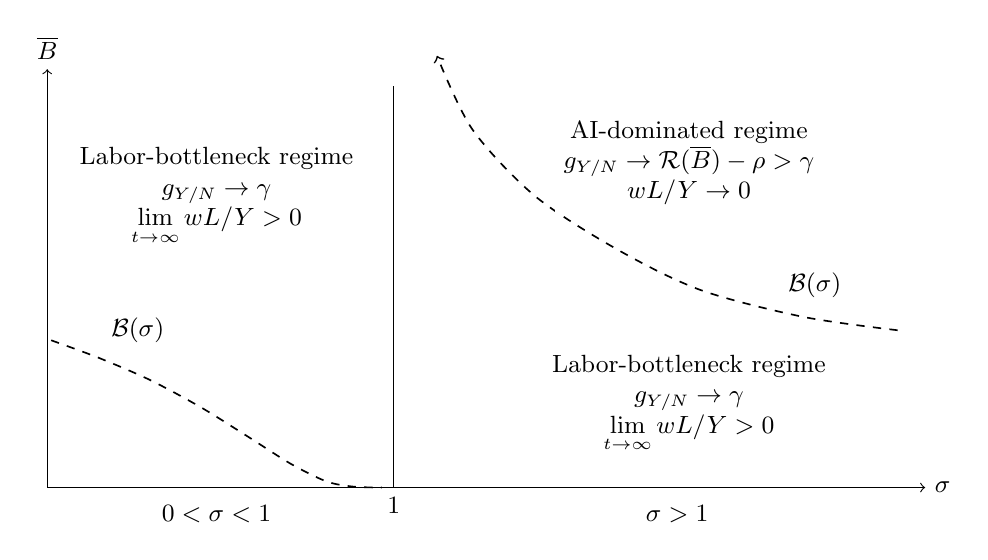
\begin{tikzpicture}[
 x=1.00cm,y=0.85cm,
 every node/.style={font=\small},
 regime/.style={align=center,inner sep=3pt,fill=white}
]
 \draw[->] (0,0) -- (11.15,0) node[right] {$\sigma$};
 \draw[->] (0,0) -- (0,6.25) node[above] {$\overline B$};
 \draw[semithick] (4.40,0) -- (4.40,6.00);
 \node[below] at (4.40,0) {$1$};
 \node[below] at (2.15,-0.12) {$0<\sigma<1$};
 \node[below] at (8.00,-0.12) {$\sigma>1$};

 % The complementary branch approaches zero as sigma approaches one
 % from below. It is not a continuation of the gross-substitutes branch.
 \draw[semithick,dashed]
  plot[smooth] coordinates
  {(0.05,2.20) (0.65,1.94) (1.30,1.61) (1.95,1.20)
   (2.55,0.76) (3.10,0.35) (3.55,0.09) (3.90,0.012)
   (4.25,0.001)};
 \node[regime] at (2.15,4.35)
  {Labor-bottleneck regime\\
   $g_{Y/N}\to\gamma$\\
   $\displaystyle\lim_{t\to\infty}wL/Y>0$};
 \node[regime] at (1.15,2.35) {$\mathcal B(\sigma)$};

 \draw[semithick,dashed,->]
  plot[smooth] coordinates
  {(10.80,2.35) (9.60,2.55) (8.30,2.95) (7.25,3.55)
   (6.20,4.35) (5.40,5.35) (4.95,6.45)};

 \node[regime] at (8.15,4.85)
  {AI-dominated regime\\
   $g_{Y/N}\to \mathcal R(\overline B)-\rho>\gamma$\\
   $wL/Y\to0$};
 \node[regime] at (8.15,1.25)
  {Labor-bottleneck regime\\
   $g_{Y/N}\to\gamma$\\
   $\displaystyle\lim_{t\to\infty}wL/Y>0$};
 \node[regime] at (9.75,3.02) {$\mathcal B(\sigma)$};
\end{tikzpicture}%
}
\caption{Constructed finite-frontier regimes. The vertical axis is linear
and the curves are schematic rather than calibrated. For $0<\sigma<1$,
$\overline B>\mathcal B(\sigma)$ is the condition for the positive-labor-share
construction in Proposition~\ref{prop:rewrite-capped-complements-existence}. For $\sigma>1$,
the curve separates the labor-bottleneck and AI-dominated equilibria in
Proposition~\ref{prop:rewrite-capped-substitutes-labor-existence}
and~\ref{prop:rewrite-capped-substitutes-existence}.}
\label{fig:rewrite-frontier-regimes}
\end{figure}


The identity $wL/Y=(1-\alpha)(1-s_X)$ translates these limits into income shares. Labor retains a positive share in the first three cases and a vanishing share in the fourth. At unit elasticity, its share is exactly $(1-\alpha)\omega_L$ at every date; correspondingly, $p_XX/Y=(1-\alpha)\omega_X$, whereas $s_X=\omega_X$. Write $\overline r=\lim_{t\to\infty}r_t$ along a constructed equilibrium. Table~\ref{tab:rewrite-finite-existence} summarizes the four cases.

\begin{table}[H]
\centering
\caption{Constructed finite-frontier equilibria}
\label{tab:rewrite-finite-existence}
\small
\begin{tabular}{@{}llll@{}}
\toprule
Elasticity & AI Efficiency & $\lim g_{Y/N}$ & $\lim wL/Y$ \\
\midrule
$0<\sigma<1$ & $\overline B>\mathcal B(\sigma)$ & $\gamma$ & Positive \\
$\sigma=1$ & Any finite $\overline B>0$ & $\gamma$ & $(1-\alpha)\omega_L$ \\
$\sigma>1$ & $\overline B<\mathcal B(\sigma)$ & $\gamma$ & Positive \\
$\sigma>1$ & $\overline B>\mathcal B(\sigma)$ & $\mathcal R(\overline B) -\rho>\gamma$ & Zero \\
\bottomrule
\end{tabular}
\end{table}

For $\sigma>1$, the strict inequalities distinguish the two equilibrium
families in Proposition~\ref{prop:rewrite-equilibrium-regimes}:
\begin{itemize}
 \item If $\mathcal R(\overline B)<\rho+\gamma$, equivalently
 $\overline B<\mathcal B(\sigma)$, the return at a vanishing labor share
 cannot sustain growth faster than effective labor. The constructed
 equilibrium retains a positive labor share, and its actual interest rate
 converges to $\rho+\gamma$, not to $\mathcal R(\overline B)$.
 \item If $\mathcal R(\overline B)>\rho+\gamma$, equivalently
 $\overline B>\mathcal B(\sigma)$, the return supports growth faster than
 effective labor even as labor's share vanishes. Along the constructed
 AI-dominated equilibrium, $r\to\mathcal R(\overline B)$ and output per
 person grows asymptotically at $\mathcal R(\overline B)-\rho>\gamma$.
 \item If $\mathcal R(\overline B)=\rho+\gamma$, the two return formulas
 coincide. This equality identifies the boundary between the strict
 regimes, but the existence proof does not cover it. It establishes
 neither existence nor nonexistence of an equilibrium at the threshold.
\end{itemize}
I use this comparison as an economic regime threshold only for $\sigma>1$.
For $\sigma<1$, $s_X\to1$ corresponds instead to AI services becoming scarce
relative to effective labor. The condition
$\overline B>\mathcal B(\sigma)$, or
$\mathcal R(\overline B)>\rho+\gamma$, is then only a sufficient condition
for the positive-labor-share construction in
Proposition~\ref{prop:rewrite-capped-complements-existence}; it does not
imply AI-dominated growth.

The proof first expresses growing quantities and shrinking efficiency gaps
in units with finite limits. For each parameter configuration covered by
the proposition, I conjecture a stationary point of these normalized
dynamics and derive its values from the model. I then construct
trajectories from every sufficiently nearby admissible initial state,
selecting $C_0,q_0$ and verifying agent optimality and both transversality
conditions. The initial stocks need not lie on a balanced-growth path.

This result is local in initial states, not in time. Closeness concerns
capital, the remaining AI-efficiency gap, and the scale of effective labor
jointly; $B_0$ close to $\overline B$ alone is not sufficient. The precise
sets and local uniqueness result are given in the proof. Existence from
arbitrary initial states and global uniqueness are not established.
These analytical limits also guide the algorithm's boundary conditions
(Appendix~\ref{app:rewrite-algorithm}), but do not determine the duration
or shape of the transition.

Across these equilibrium regimes, long-run real-wage growth exceeds $\gamma$ if and
only if labor's income share converges to zero.
Proposition~\ref{prop:rewrite-output-wage-wedge} in
Appendix~\ref{app:rewrite-proofs} derives the exact relationship between
the wage-growth premium and the decline in labor's income share.

\subsection{Raising the AI-efficiency frontier}
\label{subsec:rewrite-growth-frontier}

The constructed trajectories have convergent growth rates and a positive
limiting consumption--output ratio. Consumption and output therefore have
the same limiting growth rate. The household Euler equation gives
\begin{equation}
 \lim_{t\to\infty}\frac{\mathrm d\log(Y_t/N_t)}{\mathrm dt}
 =\lim_{t\to\infty}(g_C-n)=\overline r-\rho.
 \label{eq:rewrite-long-run-growth-return}
\end{equation}
These are limits of equilibrium transitions, not restrictions imposed on
their growth rates at every date.

\Needspace{4\baselineskip}
Holding $\sigma>1$ and all other parameters fixed, the constructed families
give the following comparative statics across finite frontiers:
\begin{equation}
 \overline r(\overline B;\sigma)=
 \begin{cases}
  \rho+\gamma,&\mathcal R(\overline B)<\rho+\gamma,\\[2pt]
  \mathcal R(\overline B),&\mathcal R(\overline B)>\rho+\gamma.
 \end{cases}
 \label{eq:rewrite-interest-frontier}
\end{equation}
Below the threshold, a larger frontier does not change the limiting
interest or growth rate. Above it,
\begin{equation}
 \frac{\partial\overline r}{\partial\overline B}
 =\frac{1-\alpha}{\alpha}
 \frac{\mathcal R(\overline B)+\delta}{\overline B}>0,
 \qquad
 \lim_{\overline B\to\infty}\overline r(\overline B;\sigma)=\infty.
 \label{eq:rewrite-interest-frontier-derivative}
\end{equation}
The limiting growth rate per person has the same derivative because it
equals $\overline r-\rho$. The two interest-rate formulas approach
$\rho+\gamma$ at the threshold, although the existence proof does not cover
equality. For $\sigma=1$, and for the constructed complementary-input
family, $\overline r=\rho+\gamma$ instead remains independent of the frontier.

\subsection{The uncapped economy and the role of the frontier}
\label{subsec:rewrite-uncapped}

The comparative static in
\eqref{eq:rewrite-interest-frontier-derivative} does not solve the economy
with an infinite AI-efficiency frontier. It first fixes a finite
$\overline B$, constructs an equilibrium, takes that
economy's long-run limit, and only then compares the resulting limits as
$\overline B$ increases. Setting $\overline B=\infty$ at the outset changes
the state equation by setting $\psi(B)=1$ and removes the bound on the
developer's state. In general,
\begin{equation}
 \lim_{\overline B\to\infty}\lim_{t\to\infty}r_t(\overline B)
 \quad\text{need not equal}\quad
 \lim_{t\to\infty}r_t(\infty),
 \label{eq:rewrite-noncommuting-limits}
\end{equation}
and the expression on the right may not exist. The initial-stock
neighborhood and the equilibrium choices of $C_0$ and $q_0$ also depend on
the frontier. Existence for every fixed finite frontier therefore does not
imply existence in the uncapped economy.

This distinction is especially important when $\sigma>1$. At high AI
efficiency, effective AI production services can replace labor. Holding
current $K,A,$ and $L$ fixed, optimized operating profit then grows
asymptotically in proportion to $KB^{(1-\alpha)/\alpha}$. Research raises
$B$, and a higher $B$ both raises operating profit and makes subsequent
research compute more productive. The capped equilibria reveal the strength
of this feedback: once the economy is in the AI-dominated regime, the
limiting interest and output-growth rates increase with $\overline B$ and
become unbounded as $\overline B\to\infty$. This divergence is evidence that
the uncapped problem may behave qualitatively differently. It is not, by
itself, proof of a finite-time singularity or of equilibrium nonexistence.
No analogous divergence appears in the finite-frontier equilibria constructed
for $\sigma\leq1$, where labor remains a long-run bottleneck. This does not
establish existence without a frontier in those cases either.

The developer's optimization problem identifies a more immediate possible
failure. Proposition~\ref{prop:rewrite-research-scale} in
Appendix~\ref{app:rewrite-proofs} shows that, in the uncapped economy,
the condition $\eta<\alpha$ makes the benefit generated by a
large research expenditure grow at most sublinearly in that expenditure on
a fixed finite horizon, while its cost grows linearly. It therefore rules out
an arbitrarily large research burst as the developer's optimal response in
that partial-equilibrium problem. If instead $\sigma>1$ and $\eta>\alpha$,
the developer can make its finite-horizon payoff arbitrarily large by
increasing an early research burst. No finite research plan maximizes its
objective. At $\eta=\alpha$, the outcome depends on the coefficients of the
leading benefit and cost terms. These results explain why $\eta<\alpha$ is a
substantive restriction, but they still do not establish an uncapped
infinite-horizon general equilibrium.

The failure when the developer's value is unbounded is economic rather than
numerical. Research compute $M$ is a use of the final good, not merely a
financial position. The household may finance a negative distribution from
the developer, but finance cannot create the real resources used in research.
Equation~\eqref{eq:rewrite-eq-kdot} requires research to compete with
consumption, inference compute, and physical investment. If every finite
research plan can be improved by choosing a larger research burst, no
allocation with finite resources can satisfy the developer's optimality
condition and the aggregate resource constraint at the same time. Such an
allocation is not an equilibrium under
Definition~\ref{def:rewrite-equilibrium}.

A different failure can occur even when the developer's value is bounded on
every finite horizon. Recursive improvement may cause $B$, output, capital,
or research expenditure to become unbounded at a finite date. I use
\emph{finite-time singularity} for this event, rather than for merely rapid
growth. A path that ends at such a date is not an equilibrium
as defined in Section~\ref{sec:rewrite-model}: it does not provide finite,
feasible allocations for every $t\geq0$, and its infinite-horizon optimality
and transversality conditions are not defined. The analysis in this paper
does not prove that every uncapped trajectory with $\sigma>1$ reaches such a
singularity. It also does not rule out an uncapped equilibrium that remains
finite at every finite date. Explosive-growth mechanisms in
\citet{nordhaus2021} and \citet{davidsonetal2026} motivate this question but
do not replace the missing equilibrium argument for the present model.

I therefore use a finite frontier as an analytical continuation device, not
as an estimate of a permanent technological ceiling. For each finite
$\overline B$, the term $1-B/\overline B$ keeps AI efficiency in a bounded
state space and makes it possible to establish and compute an equilibrium.
I then raise the frontier and examine how the equilibrium regime, growth,
interest rates, and income shares change. This strategy separates results
that hold for every fixed finite frontier from claims about an uncapped
economy. If the capped equilibria fail to converge, or their limiting growth
rates diverge, the correct conclusion is that this continuation does not
produce an uncapped equilibrium---not that a finite-time singularity has
already been proved.
